\documentclass [a4paper,11pt]{article}
\usepackage{amssymb}
\usepackage{amsthm}
\usepackage[intlimits]{amsmath}
\usepackage[polish]{babel}
\usepackage[utf8]{inputenc}
\usepackage[T1]{fontenc}
\frenchspacing
\usepackage{indentfirst}
\usepackage{graphicx}
\usepackage{subfig}
\usepackage{mathptmx}
\usepackage{geometry}
\usepackage{wrapfig}
\sloppy

\usepackage{array}
\newcolumntype{L}[1]{>{\raggedright\let\newline\\\arraybackslash\hspace{0pt}}m{#1}}
\newcolumntype{C}[1]{>{\centering\let\newline\\\arraybackslash\hspace{0pt}}m{#1}}
\newcolumntype{R}[1]{>{\raggedleft\let\newline\\\arraybackslash\hspace{0pt}}m{#1}}
\begin{document}
\newgeometry{tmargin=2cm, bmargin=2cm, lmargin=2cm, rmargin=2cm}

%----------- tabela nagłówkowa---------------------- %
\begin{table}[]
\centering
\begin{tabular}{lllllll}
\cline{1-6}
\multicolumn{1}{|c|}{\begin{tabular}[c]{@{}c@{}}EAiIB\\ Informatyka\end{tabular}}              & \multicolumn{2}{l|}{\begin{tabular}[c]{@{}l@{}}Autor 1\\ Autor 2\end{tabular}}                                                                                                & \multicolumn{1}{c|}{\begin{tabular}[c]{@{}c@{}}Rok\\ II\end{tabular}}          & \multicolumn{1}{c|}{\begin{tabular}[c]{@{}c@{}}Grupa\\ V\end{tabular}}            & \multicolumn{1}{c|}{\begin{tabular}[c]{@{}c@{}}Zespół\\ II\end{tabular}}      &  \\ \cline{1-6}
\multicolumn{1}{|c|}{\begin{tabular}[c]{@{}c@{}}Pracownia\\ FIZYCZNA\\ WFiIS AGH\end{tabular}} & \multicolumn{4}{l|}{\begin{tabular}[c]{@{}l@{}}Temat:\\ \textbf{Elektroliza} \end{tabular}}                                                                                                                                                                                                                                            & \multicolumn{1}{l|}{\begin{tabular}[c]{@{}l@{}}nr ćwiczenia:\\35\end{tabular}} &  \\ \cline{1-6}
\multicolumn{1}{|l|}{\begin{tabular}[c]{@{}c@{}}Data wykonania:\\ 7.10.2015\end{tabular}}      & \multicolumn{1}{c|}{\begin{tabular}[c]{@{}c@{}}Data oddania:\\ 14.10.2015\end{tabular}} & \multicolumn{1}{l|}{\begin{tabular}[c]{@{}l@{}}Zwrot do poprawki:\\ \phantom{data poprawki}\end{tabular}} & \multicolumn{1}{l|}{\begin{tabular}[c]{@{}l@{}}Data oddania:\\  \phantom{data oddania}\end{tabular}} & \multicolumn{1}{l|}{\begin{tabular}[c]{@{}l@{}}Data zaliczenia:\\  \phantom{data zaliczenia}\end{tabular}} & \multicolumn{1}{l|}{\begin{tabular}[c]{@{}l@{}}OCENA:\\ \phantom{ocena}\end{tabular}}       &  \\ \cline{1-6}
                                                                                               &                                                                                         &                                                                                     &                                                                                &                                                                                   &                                                                               & 
\end{tabular}
\end{table}

\section{Cel ćwiczenia}

Wyznaczanie równoważnika  elektrochemicznego    miedzi    oraz    stałej    Faradaya w doświadczeniu z elektrolizą wodnego roztworu $\text{CuSO}_4$

\section{Wstęp}
Charakterystyczną grupę przewodników prądu elektrycznego stanowią elektrolity. Są to przeważnie wodne roztwory zasad, kwasów i soli. Przy rozpuszczaniu kryształu wiązania jonowe pękają i atomy przechodzą do roztworu w postaci jonów poruszających się bezwładnie w roztworze. Jeśli przez roztwór ten przepuścimy prąd elektryczny, to ruch jonów staje się uporządkowany. Kationy zdążają do ujemnej elektrody, aniony do katody. Przepływowi prądu towarzyszy zobojętnianie jonów na elektrodach i wydzielanie się substancji na elektrodach. Proces ten nazywamy elektrolizą.

W celu zobojętnienia naładowanego elektrycznie jonu, musi przepłynąć ładunek równy: $ w \cdot e$, gdzie $w$ to wartościowość jonu. 
 Dla przykładu jony w związku używanym w doświadczeniu ( $\text{CuSO}_4$) mają wartościowość $w = 2$. 
Liczba wydzielonych na elektrodzie atomów $N$ jest równa stosunkowi wartości dostarczonego ładunku do ładunku pojedynczego jonu:
\begin{equation}
N = \frac{I t}{w e}
\end{equation}

Aby otrzymać masę powstałych atomów trzeba wartość tę podzielić przez liczbę Avogadro i pomnożyć przez masę molową.
\begin{equation}
m = N \frac{\mu}{N_A} = \frac{\mu}{ w e N_A} It
\label{masa}
\end{equation}
Zgodnie z I prawem Faradaya wydzielona masa jest proporcjonalna do wartości przepływającego prądu oraz czasu:
\begin{equation}
m = k I t
\label{I_prawo}
\end{equation}
Porównując wzory (\ref{I_prawo}) i (\ref{masa}) otrzymujemy wzór na współczynnik proporcjonalności $k$ zwany elektrochemicznym równoważnikiem substancji:
\begin{equation}
k = \frac{\mu}{w e  N_A}
\label{wspol-k}
\end{equation}
 Iloczyn $e N_A$ to stała Faradaya Jest to wartość stała. Przekształcając wzór (\ref{wspol-k}) otrzymamy wzór na stałą Faradaya oraz wartość ładunku elementarnego
 
  \begin{equation}
  F = e N_A =  \frac{\mu}{w k} 
  \label{stala_Faradaya_wzór}
  \end{equation}
 

\section{Układ pomiarowy}


\subsubsection*{Przyrządy}
\begin{itemize}
\item Naczynie do elektrolizy siarczanu miedzi $\text{CuSO}_4$ z miedzianymi elektrodami w kształcie
równoległych płyt, oddalonych od siebie o kilka centymetrów (rys. 1).
\item Zasilacz napięcia stałego
\item Amperomierz
\item Opornica suwakowa
\item Waga elektroniczna
\end{itemize}

\begin{figure}[h!]
\centering
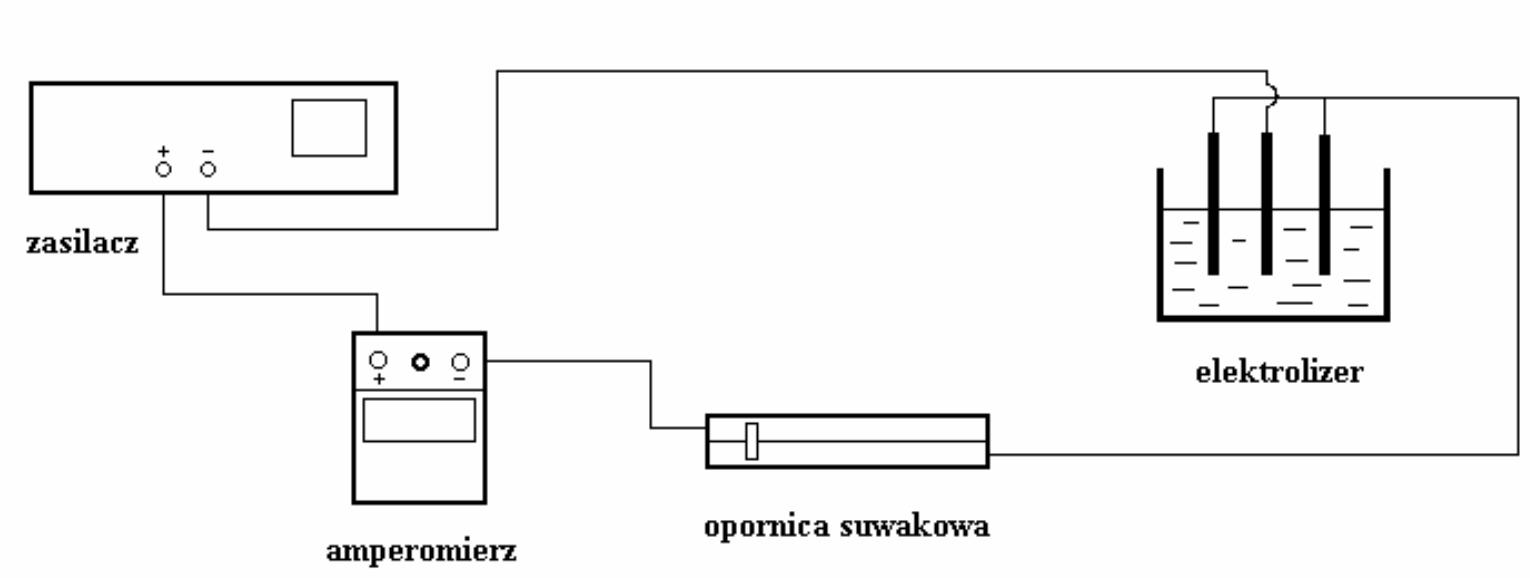
\includegraphics[width=0.7\linewidth]{./uklad}
\caption{Schemat obwodu elektrycznego}
\label{fig:uklad}
\end{figure}


\section{Wyniki pomiarów}
\begin{tabular}{lrlll}
czas elektrolizy               & $t$ & = & 35 & min  \\ 
 natężenie prądu               &  $I$ & = & 0,65 & A \\ 
 masa katody przed elektrolizą &  $m_1$ & = & 113,262 & g \\ 
  masa katody po elektrolizie  &   $m_2$ & = & 113,715 & g\\ 
 masa wydzielonej miedzi       &  $m = m_2 - m_1$& = & 0,453 & g \\ 
 masa anod przed elektrolizą   &   $M_1$ & = &214,646 & g\\ 
 masa anod po elektrolizie     &   $M_2$ & = &214,197 & g\\ 
zmiana masy anod               &  $M = M_2 - m_1$& = & 0,451 & g \\  
\end{tabular} 

\subsection*{Dane określające niepewność przyrządów:}
\begin{tabular}{lrlll}
Klasa amperomierza              & &  & 0,5 &   \\ 
Używany zakres amperomierza               &   &  & 0,75 & A \\ 
Niepewność graniczna wagi (znamionowa)&  $\Delta m$ & = & 0,001 & g \\ 
 Niepewność pomiaru masy &   $u(m)$& = & 0,005 & g\\  
\end{tabular} 

\section{Opracowanie wyników}
Przekształcając wzór (\ref{I_prawo}) możemy obliczyć współczynnik elektrochemiczny $k$ :
\begin{equation}
k = \frac{m}{I t} = \frac{453 \cdot 10^{-3}}{65 \cdot 10^{-2} \cdot 21 \cdot 10^2} = \frac{453}{65 \cdot 21} \cdot 10^{-3} \approx 0,3319 \cdot 10^{-3} \left[  \frac{g}{A \cdot s}\right] 
\label{k_obliczone} 
\end{equation}

Korzystając z otrzymanej w (\ref{k_obliczone})  wartości współczynnika  $k$ i  wzoru (\ref{stala_Faradaya_wzór}),
obliczamy eksperymentalną wartość stałej Faradaya;
\begin{equation}
F = \frac{\mu}{w k} = \frac{63,58 }{2 \cdot 33,19 \cdot 10^{-5}} \approx 95782   \left[  \frac{C}{mol}\right] 
\label{F_obliczone} 
\end{equation}

Korzystając z otrzymanej w (\ref{F_obliczone})  wartości stałej Faradaya  $F$, obliczamy eksperymentalną wartość ładunku elementarnego :
\begin{equation}
e = \frac{F}{N_A} = \frac{9,5782 \cdot 10^4}{6,0222 \cdot 10^{23}} \approx 1,5905 \cdot 10^{-19}   \left[  C \right] 
\label{e_obliczone} 
\end{equation}

\section{Obliczanie niepewności pomiarowej}
Niepewność pomiaru czasu uznajemy za pomijalnie małą (niepewność względna znacznie poniżej $ 1 \% $)
 
Niepewność pomiaru masy miedzi wydzielonej podczas elektrolizy przyjmujemy jako:

\begin{equation*}
u(m) = 0,005 g
\end{equation*}

ze względu na możliwość niedokładnego wysuszenia elektrod po procesie elektrolizy.


Niepewność wartości ładunku elektrycznego, który przepłynął przez elektrolit
\begin{equation*}
u(I) = \frac{\text{klasa amperomierza} \cdot \text{zakres}}{100} = 3,75 \cdot 10^{-3} [A]
\end{equation*}

\begin{equation*}
u(Q) = t \cdot u(I) = 3,75 \cdot 10^{-3} \cdot 2,1 \cdot 10^3 = 7,875 [C]
\end{equation*}

\subsubsection*{Niepewność względna i bezwzględna  równoważnika elektrochemicznego}  

\begin{equation*}
\frac{u(k)}{k} = \sqrt{\left[\frac{u(m)}{m} \right]^2 + \left[\frac{u(I)}{I} \right]^2 } = \sqrt{\left[\frac{ 0,005}{0,453} \right]^2 + \left[\frac{0,00375}{0,65} \right]^2 } \approx 0,0125
\end{equation*}

\begin{equation*}
u(k) = \frac{u(k)}{k} \cdot k =  0,0125 \cdot 0,3319 \cdot 10^{-3} \approx 0,0042 \cdot 10^{-3}  \left[  \frac{g}{A \cdot s}\right] 
\end{equation*}

\subsubsection*{Niepewność względna i bezwzględna  stałej Faradaya oraz ładunku elementarnego}

\begin{equation*}
\frac{u(F)}{F} = \sqrt{\left[\frac{u(\mu)}{\mu} \right]^2 + \left[\frac{u(k)}{k} \right]^2 } = \sqrt{\left[\frac{u(k)}{k} \right]^2 } = \frac{u(k)}{k}  =   \frac{u(e)}{e}
\end{equation*}

\begin{equation*}
u(F) = F \frac{u(k)}{k}  =  95782  \cdot  0,0125 \approx 1193  \left[  \frac{C}{mol}\right] 
\end{equation*}

\begin{equation*}
u(e) = e \frac{u(k)}{k}  =  1,5905 \cdot 10^{-19}  \cdot  0,0125 \approx 0,0198 \cdot 10^{-19} [C] 
\end{equation*}

\section{Podsumowanie wyników}



\begin{tabular}{|C{0.12\linewidth}|C{0.12\linewidth}|C{0.14\linewidth}|C{0.12\linewidth}|C{0.12\linewidth}|C{0.12\linewidth}|}
\hline  & wartość tablicowa  & wartość wyznaczona w eksperymencie & różnica & niepewność  & niepewność względna [\%]  \\ 
\hline $k \left[  \frac{mg}{A \cdot s}\right]$ & 0,3294  & 0,3319  & 0,0025  & 0,0042  & 1,25  \\ 
\hline $F \left[  \frac{C}{mol}\right]$ & 96500 & 95782  & 718  & 1193  & 1,25  \\ 
\hline $e [10^{-19} C]$ & 1,6022   & 1,5905    & 0,0117    & 0,0198   & 1,25  \\ 
\hline 
\end{tabular} 
\section{Wnioski}
\begin{itemize}
\item Wyznaczone eksperymentalnie wartości są zgodne z wartościami tablicowymi w granicach niepewności pomiarowych, co świadczy o poprawności metody
\item Uzyskane niepewności względne są dosyć małe (ok 1\%) co świadczy o dokładności metody
\item Różnica pomiędzy zmianą masy anod a masą wydzielonej miedzi mieści się w granicach niepewności pomiarowych
%\item Największe trudności w doświadczeniu sprawia delikatne osuszenie katody po elektrolizie, aby nie zetrzeć części wydzielonej miedzi

 
\end{itemize}

\end{document}